\documentclass[tikz,border=4mm]{standalone}
\usepackage[T1]{fontenc}
\usepackage{helvet}
\renewcommand{\familydefault}{\sfdefault}
\usetikzlibrary{arrows.meta,positioning,fit,backgrounds}

\begin{document}
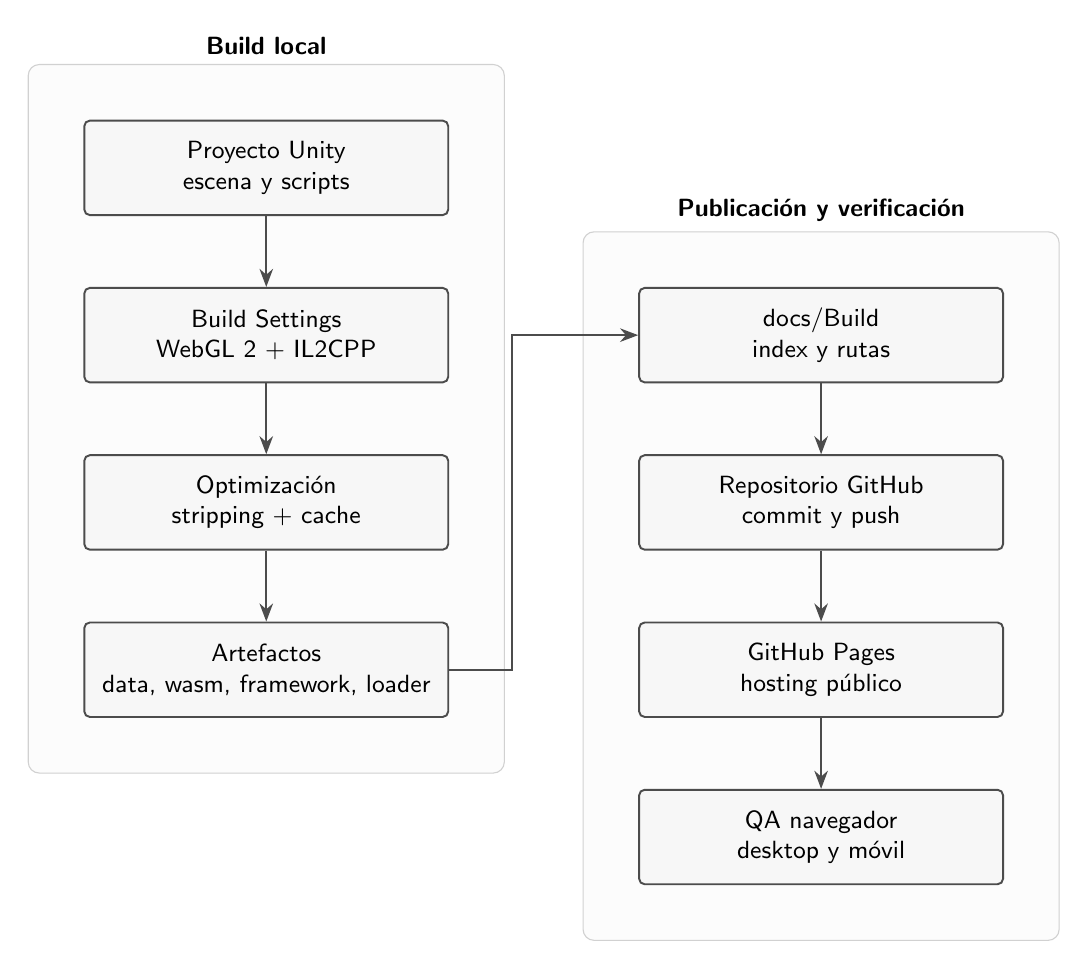
\begin{tikzpicture}[
  font=\sffamily\small,
  node distance=9mm and 24mm,
  box/.style={
    draw=black!70,
    rounded corners=2pt,
    line width=0.7pt,
    fill=black!3,
    align=center,
    inner sep=6pt,
    minimum height=12mm,
    text width=42mm
  },
  lane/.style={draw=black!18, rounded corners=4pt, fill=black!1, inner sep=7mm},
  arrow/.style={-{Stealth[length=2.3mm]}, line width=0.65pt, draw=black!70}
]

\node[box] (project) {Proyecto Unity\\escena y scripts};
\node[box, below=of project] (settings) {Build Settings\\WebGL 2 + IL2CPP};
\node[box, below=of settings] (opt) {Optimizaci\'on\\stripping + cache};
\node[box, below=of opt] (artifacts) {Artefactos\\data, wasm, framework, loader};

\node[box, right=of settings] (docs) {docs/Build\\index y rutas};
\node[box, below=of docs] (repo) {Repositorio GitHub\\commit y push};
\node[box, below=of repo] (pages) {GitHub Pages\\hosting p\'ublico};
\node[box, below=of pages] (qa) {QA navegador\\desktop y m\'ovil};

\draw[arrow] (project) -- (settings);
\draw[arrow] (settings) -- (opt);
\draw[arrow] (opt) -- (artifacts);
\draw[arrow] (artifacts.east) -- ++(8mm,0) |- (docs.west);
\draw[arrow] (docs) -- (repo);
\draw[arrow] (repo) -- (pages);
\draw[arrow] (pages) -- (qa);

\begin{scope}[on background layer]
  \node[lane, fit=(project)(settings)(opt)(artifacts), label={[font=\sffamily\bfseries\small]above:Build local}] {};
  \node[lane, fit=(docs)(repo)(pages)(qa), label={[font=\sffamily\bfseries\small]above:Publicaci\'on y verificaci\'on}] {};
\end{scope}

\end{tikzpicture}
\end{document}
